\subsubsection{Advanced thread scheduling}

The \emph{main goal} of this section is to show how a CUDA kernel uses hardware execution resources: thread block allocation to execution resources, execution resource capacity constraints, and zero-overhead thread scheduling.

\highspace
In general, \textbf{CUDA thread blocks execute independently and can run in any order}. The hardware is \textbf{free to assign blocks to any processor at any time}. This flexibility allows the GPU to optimize resource utilization and balance the load. A kernel (the function that runs on the GPU) scales to any number of parallel processors. This means that the same code can run efficiently on GPUs with different numbers of cores.

\highspace
\begin{wrapfigure}{r}{0.35\textwidth}
    \centering
    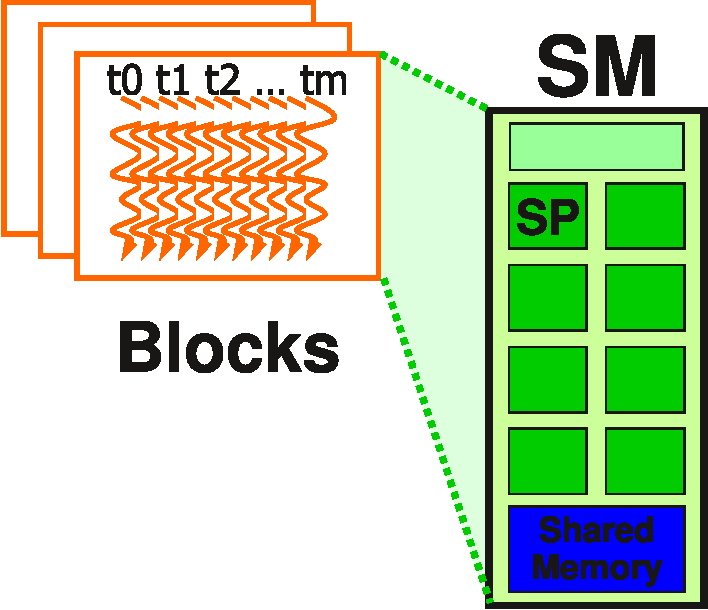
\includegraphics[width=0.34\textwidth]{img/executing-thread-blocks-1.pdf}
\end{wrapfigure}
Thread blocks are the basic unit of work in CUDA and are assigned to SMs in block granularity (as we saw in Chapter \ref{subsubsection: Running a CUDA program on a GPU}). This means that a \textbf{thread block cannot be split across multiple SMs, but is executed entirely within a single SM}. Each SM has a \emph{limit} on the number of threads and thread blocks it can support simultaneously. For example, the \textbf{Volta SM can handle up to 2048 threads}. The number of blocks an SM can hold depends on the number of threads per block:
\begin{itemize}
    \item If a block has 256 threads, up to 8 blocks can fit ($256 \times 8 = 2048$ threads).
    \item If a block has 512 threads, only 4 blocks can fit ($512 \times 4 = 2048$ threads).
\end{itemize}
The \textbf{SM manages the indexes of the threads and blocks assigned to it}, enabling scheduling and execution.

\highspace
\begin{flushleft}
    \textcolor{Green3}{\faIcon{bookmark} \textbf{Von Neumann model with SIMD units}}
\end{flushleft}\index{Von Neumann model with SIMD units}
The \textbf{Von Neumann Model} consists of a Control Unit, ALU (Arithmetic Logic Unit), Registers, Memory, and I/O components that work in a sequential manner. However, when we \textbf{integrate SIMD} (Single Instruction, Multiple Data) units into the model, we add the \textbf{ability to process multiple data items simultaneously using a single instruction}.

\highspace
As we have explained in the section \ref{subsubsection: Single Instruction, Multiple Data (SIMD) processor} page \pageref{subsubsection: Single Instruction, Multiple Data (SIMD) processor}, SIMD allows the same operation to be performed on multiple pieces of data in parallel. This means a Control Unit (CU) sends the same instruction to multiple ALUs, each working on different data at the same time.

\newpage

\begin{flushleft}
    \textcolor{Green3}{\faIcon{bookmark} \textbf{Von Neumann model with SIMD units in GPUs}}
\end{flushleft}
The \textbf{architecture uses SIMD units to execute multiple threads in parallel}, making GPUs highly efficient at tasks involving large data sets, such as image processing, matrix multiplication, and other data-parallel computations.

\highspace
\textbf{Warps} (groups of 32 threads) are \textbf{executed in a SIMD fashion}. \textbf{All threads in a warp perform the same operation, but on different pieces of data}. This is critical for speeding up computations that need to process large amounts of data in parallel. SIMD capabilities allow GPUs to efficiently handle large numbers of parallel tasks, making them far more powerful than traditional CPUs for certain workloads, such as graphics rendering and scientific computing.

\begin{figure}[!htp]
    \centering
    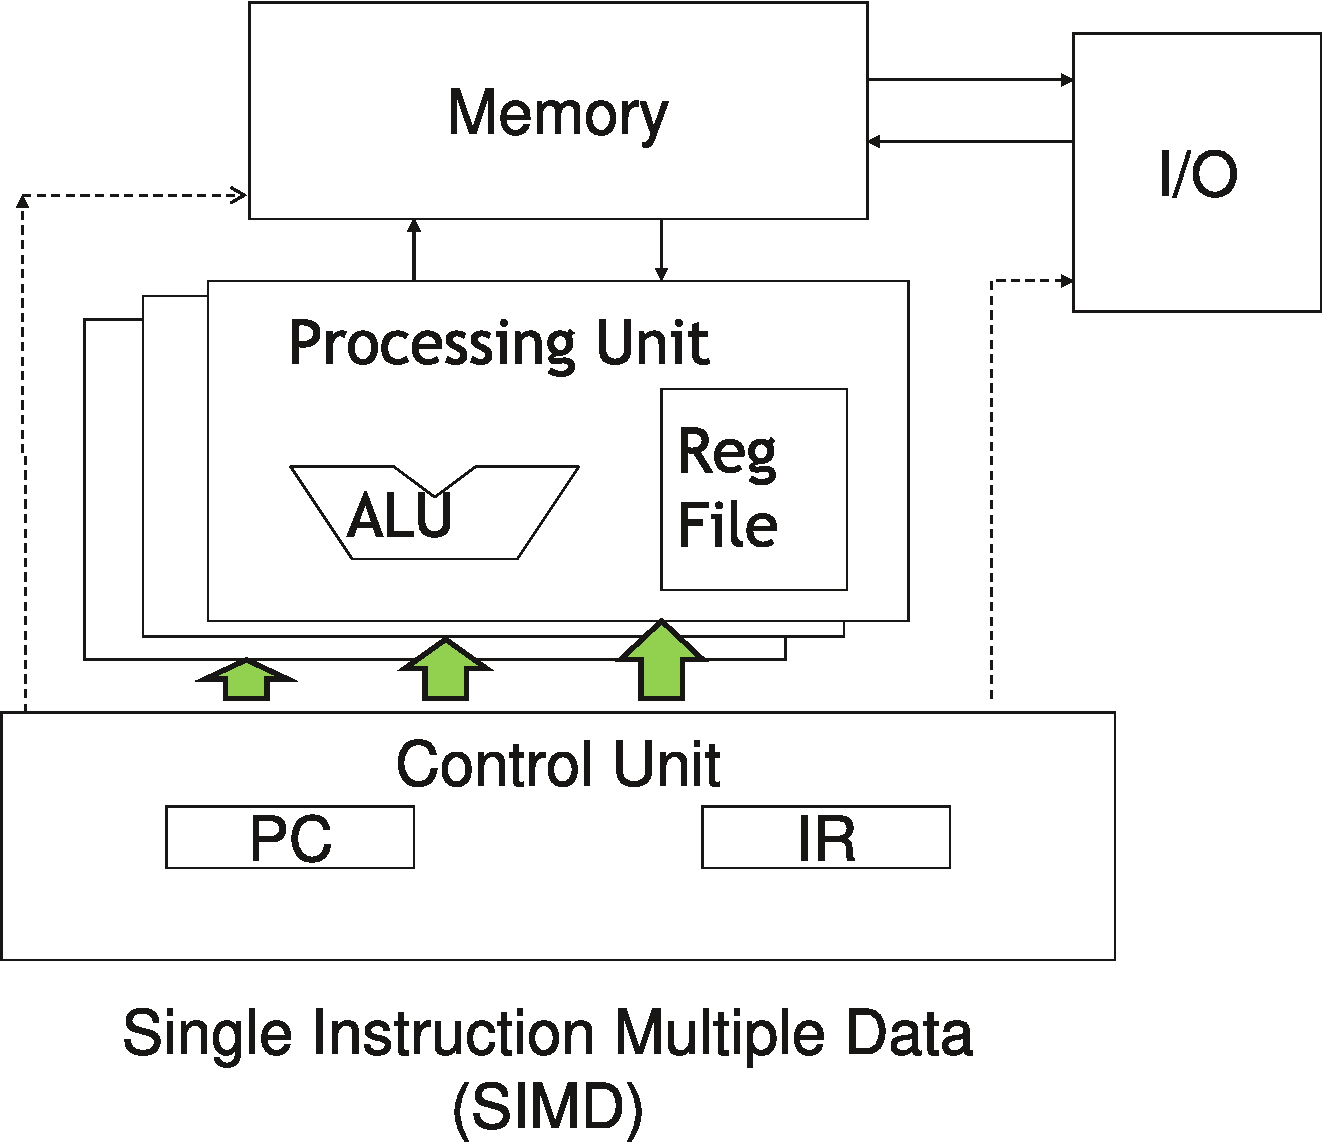
\includegraphics[width=.6\textwidth]{img/von-neumann-model-with-simd-1.pdf}
    \caption{Von Neumann model with SIMD units.}
\end{figure}

\noindent
However, these features are implementation choices, not part of the CUDA programming model. Therefore, future GPUs may have different numbers of threads in each warp.

\highspace
\begin{examplebox}[: Warp]
    If 3 blocks are assigned to a Streaming Multiprocessor (SM) and each block has 256 threads, how many warps are there in an SM?

    Since each warp is made up of 32 threads, if a block is made up of 256 threads, then 8 warps are required for each block:
    \begin{equation*}
        \dfrac{\text{Threads per block}}{\text{Threads per warp}} = \dfrac{256}{32} = 8
    \end{equation*}
    Since the number of blocks to be allocated is 3, if each block requires 8 warps, there are $8 \times 3 = 24$ warps inside a single SM.
\end{examplebox}

\newpage

\begin{flushleft}
    \textcolor{Green3}{\faIcon{book} \textbf{Zero-Overhead Warp Scheduling}}\cite{EECS570Lecture5ZeroOverheadWarpScheduling}
\end{flushleft}
\definition{Zero-Overhead Warp Scheduling} is a feature of NVIDIA's GPUs that allows \textbf{efficient management of thread execution} without significant performance penalties. This mechanism is obviously \textbf{implemented in the Streaming Multiprocessor architectures}.

\begin{itemize}
    \item \important{Warp Status}. Each warp has a state that can be:
    \begin{itemize}
        \item \textbf{Eligible}: the warp is ready to execute its next instruction because all the \emph{necessary operands are available} (ready for consumption).
        \item \textbf{Not Eligible}: the warp cannot execute its next instruction because it is \emph{waiting for operands or other resources}.
        \item \textbf{Busy}: the warp is \emph{currently running and executing instructions}.
    \end{itemize}
    Each warp also has an associated \textbf{priority value}.

    \item The scheduler has a \important{Prioritized Scheduling Policy}, so it selects:
    \begin{enumerate}
        \item \textbf{Highest Priority and Eligible}: the scheduler first selects warps that have the highest priority and are eligible for execution.
        \item \textbf{Eligible Warps}: if no high-priority warps are eligible, the scheduler then selects from the pool of eligible warps.
    \end{enumerate}

    \item \important{Execution Context Switching}. After that the scheduler choose a warp to run, \emph{how it can change the execution context from a warp to another?}
    \begin{itemize}
        \item Before giving the answer, it is necessary to understand that the \definition{Execution Context} \textbf{contains the state of all threads in a warp}, such as Program Counters, register values, and other information necessary for execution. This context is \textbf{\underline{stored in hardware} resources dedicated to each warp}.
        
        \item Thus zero-overhead warp scheduling takes advantage of the power of the hardware. When the warp \textbf{scheduler decides to switch} from one warp to another (to hide latency or because a warp is waiting for data), it does not need to save and restore context to and from memory. Instead, \textbf{it simply switches the execution state to the context of another warp, which is already stored in dedicated hardware}.
    \end{itemize}
    This means that the switching process is very fast and has virtually no overhead, hence the term \dquotes{zero-overhead}!

    In other words, \textbf{since all the necessary state information is already stored in the hardware, this switch is instantaneous and doesn't involve the overhead of saving/loading data to/from memory}.
\end{itemize}

\begin{flushleft}
    \textcolor{Green3}{\faIcon{check-circle} \textbf{Advantages}}
\end{flushleft}
\begin{itemize}
    \item \textcolor{Green3}{\textbf{Efficiency}}. By leveraging hardware resources for context storage, CUDA ensures that switching between warps incurs virtually no overhead.
    
    \item \textcolor{Green3}{\textbf{Latency Hiding}}. This efficient scheduling helps hide latencies and keeps the GPU's computational resources fully utilized, leading to high performance.
\end{itemize}

\newpage

\begin{examplebox}[: Matrix Multiplication on Volta Architecture]\label{examplebox: Matrix Multiplication on Volta Architecture}
    This example illustrates the impact of different block sizes on thread utilization when performing matrix multiplication using NVIDIA's Volta GPU architecture.

    With the term \textbf{Block Granularity} we refer to the \textbf{number of threads per block}. \textbf{Choosing the right block size is crucial for maximizing the efficiency of GPU resources}.

    \begin{itemize}
        \item In general, each Streaming Multiprocessor (SM) on the Volta architecture can handle up to 2048 threads.
        \item $4 \times 4$ Threads per Block:
        \begin{itemize}
            \item \textbf{Threads per Block}: 16 threads ($4 \times 4$).
            \item \textbf{Blocks per SM}: the GPU can accommodate up to 32 blocks per SM.
            \item \textbf{Utilization}: 16 threads per block mean 2048 threads would fill 128 blocks. However, since an SM can only accommodate up to 32 blocks at a time, only 512 threads will be utilized per SM (16 threads/block $\times$ 32 blocks), leading to under-utilization of available threads!
        \end{itemize}

        \item $8 \times 8$ Threads per Block:
        \begin{itemize}
            \item \textbf{Threads per Block}: 64 threads ($8 \times 8$).
            \item \textbf{Blocks per SM}: with 2048 threads per SM, up to 32 blocks of 64 threads each can be allocated per SM (2048 threads per SM $\div$ 64 threads per block).
            \item \textbf{Utilization}: this setup can utilize the full capacity of 2048 threads per SM, provided other resource limitations (such as shared memory or registers) are not a constraint.
        \end{itemize}

        \item $30 \times 30$ Threads per Block:
        \begin{itemize}
            \item \textbf{Threads per Block}: 900 threads ($30 \times 30$).
            \item \textbf{Blocks per SM}: with 2048 threads per SM, only two blocks of 900 threads each can be accommodated, resulting in 1800 threads (2 $\times$ 900), which is less than the SM's maximum capacity.
            \item \textbf{Utilization}: this configuration also leads to under-utilization because it does not utilize the full 2048 thread capacity.
        \end{itemize}
    \end{itemize}
\end{examplebox}

\newpage

The example on page \pageref{examplebox: Matrix Multiplication on Volta Architecture} shows some important points to emphasize:
\begin{itemize}
    \item \textbf{Choosing Block Size}: choosing the optimal block size is critical to maximizing GPU efficiency. In the previous example, a block size of $8 \times 8$ allows full utilization of the SM's thread capacity.
    \item \textbf{Resource Constraints}: when choosing a block size, we must also consider other resource limitations, such as shared memory and registers, which can affect the number of threads and blocks that can be scheduled on an SM.
\end{itemize}
